In this section we evaluate the performance of our optimizations by conducting
experiments on the TPC-H benchmark. 

\subsection{Methodology}

\head{Experimental setup.}
We run all benchmarks under Ubuntu 16.04.6 LTS on a server which has 4 Intel
Xeon E7-4850 2.00GHz (total 40 cores with 80 threads) and 128 GB RAM.
We use GCC compiler with the version \textit{v8.1.0} to compile the generated C
code after optimizations with a maximum optimization option \texttt{-O3} and
enabled \texttt{-march=native}.
We use the latest MonetDB \cite{IdreosS2012} released as \textit{Apr2019} with
version v11.33.3, as a baseline to compare with the following HorseIR versions:
(1) HorseIR-noopt: a naive version without any optimizations;
(2) HorseIR-opt1 : an optimized version with element-wise and pattern-based
fusion enabled as presented in the previous work~\OldPaper; and
(3) HorseIR-opt2 : optimization uses the approach presented in this paper.

\head{Execution time.}
Our results present the core execution time of the database query. That is, compilation time, the time to load the input data into memory and the time to output results are not considered, as we want to zoom on the effects of the optimization.  
The results present the average over 15 executions for each query.

% \head{Micro-benchmarks.}

\head{TPC-H SQL benchmarks.}
TPC-H \cite{TPCH2017} is a widely used SQL benchmark suite for analytical data
processing simulating real Business to Consumer (B2C)
database applications. The database has 8 tables over which 22 queries are
defined.  The database size can be varied by indicating a  \textit{scale factor} (SF).
For example, a scale factor of 1 (i.e. SF1) means 1GB of input
data. With an increasing scale factor, (nearly) each of the tables holds more
data records. Our results are for SF1 but initial results on larger scale
factors show similar results.

For this paper, we have selected 8 of the 22 queries (q1/4/6/12/14/16/19/22). These are the queries where the basic built-in functions that we aim to fuse have a major impact on the query execution time. In particular, these queries have a maximum of 2 joins. Joins are very expensive, and in queries with more than 2 joins, the join execution takes up most of the time, thus, the optimizations presented in \OldPaper and in this paper have less impact.   Future work will look more closely at fusion potential for join operations.  

%% In our experiments, we use a number of SFs growing exponentially, i.e.
%% SF1/2/4/8/16, to test the scalability of the generated parallel code.

% \subsection{Micro-benchmarks Results}

\subsection{Execution Time Results}

\begin{figure*}[htbp]
\centering
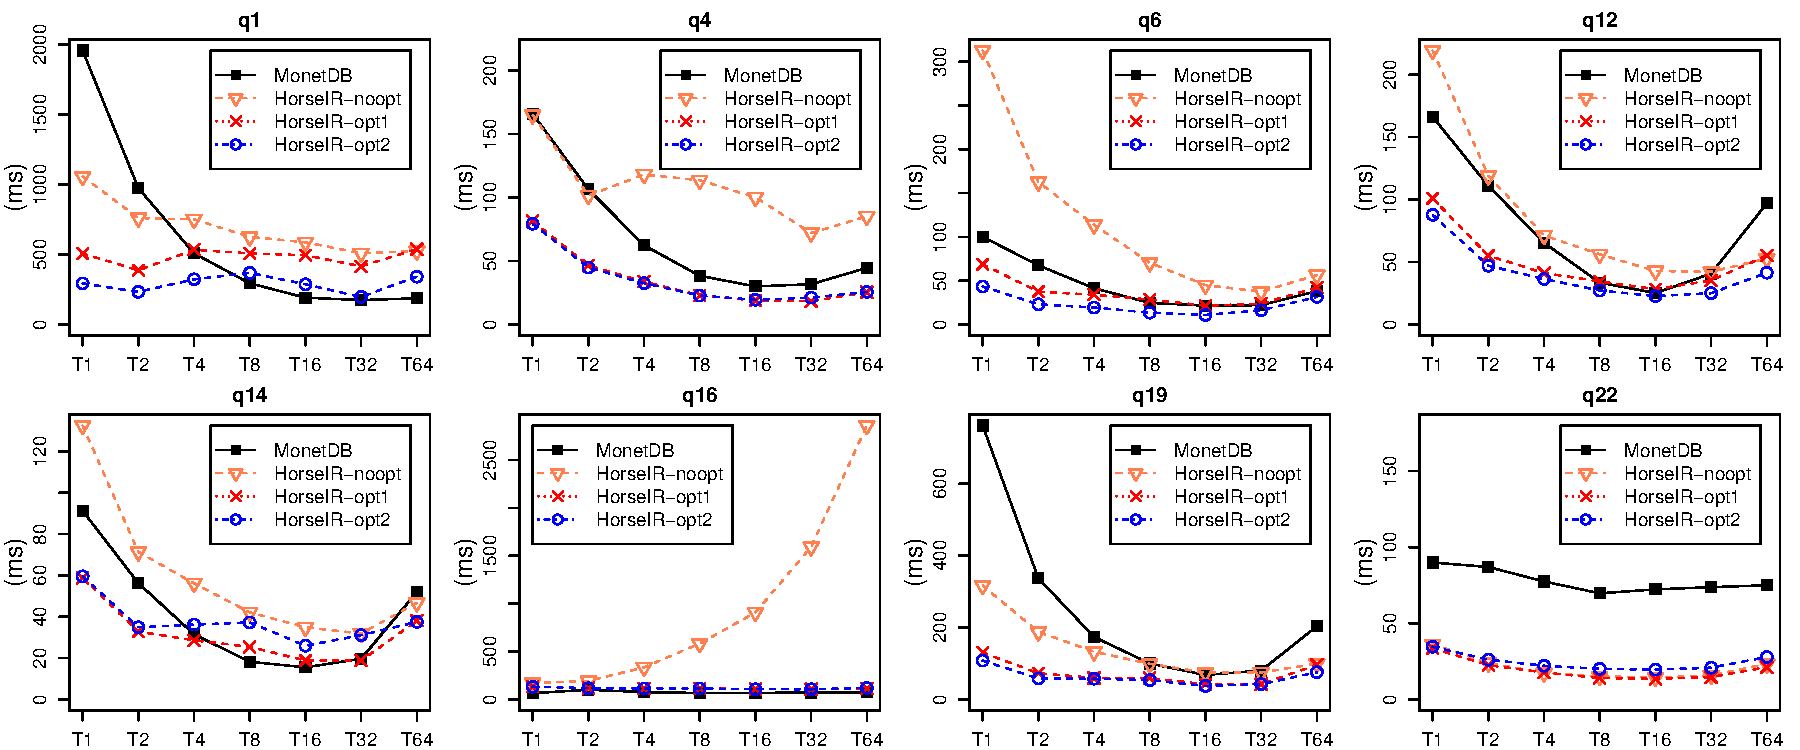
\includegraphics[width=\textwidth]{./src/figure/sf1-v2.pdf}
\caption{The result of TPC-H queries with 1GB input data (SF1).}
\label{fig:tpch_result}
\end{figure*}


\refFig{fig:tpch_result} shows the execution times using MonetDB, HorseIR-noopt,
HorseIR-opt1, and HorseIR-opt2 on SF1 with increasing number of threads. 
Execution time generally decreases with increasing number of threads up to a
thread threshold except for q16. The sweet spot for both MonetDB and HorseIR
where the best performance is achieved, is at around 16 threads. Thus, using
parallel execution is beneficial for most of the queries. The problem with q16
is that it has many cells (18314) with only a very small vector in each cell
(average size 6.5). Thus, q16 cannot take advantage of parallelization as it
focuses on the vectors in the cells. 

HorseIR-noopt has the worst performance in most cases showing that optimization
techniques are crucial when trying to exploit array-based languages for query
execution. The two HorseIR-opt versions are generally not as sensitive to the
number of threads as MonetDB, which shows quite bad performance for many
queries when there are only a few threads. 
When looking only at the optimal thread level around 16, MonetDB shows the best
performance for one query, HorseIR-opt1 for one query, HorseIR-opt2 for two
queries, HorseIR-opt1 and HorseIR-opt2 for two queries, and all three behave
very similarly for two queries. That is, there are only 2 queries where our
approach is worse than one of the other approaches, and that only by a small
margin.

\begin{figure}[htbp]
\centering
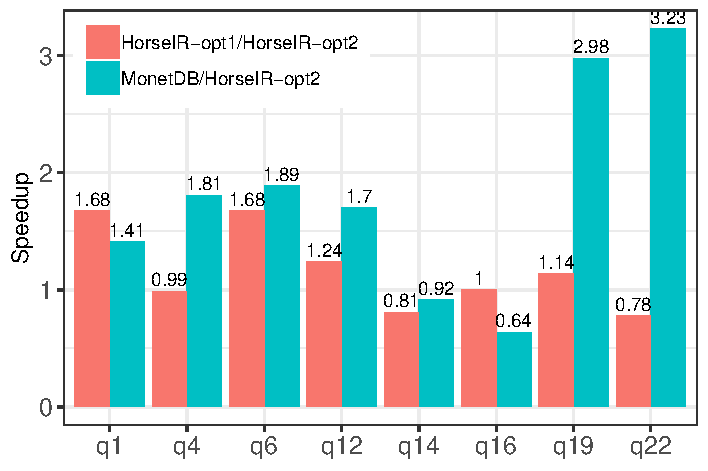
\includegraphics[width=.9\columnwidth]{./src/figure/sf1-speedup.pdf}
\caption{Geometric means of TPC-H queries with 1GB input data (SF1).}
\label{fig:tpch_sf1_speedup}
\end{figure}

In order to better understand the performance benefit of our approach across all thread levels, 
\refFig{fig:tpch_sf1_speedup}  presents  the geometric mean for the comparison
between HorseIR-opt2 in regard to HorseIR-opt1 and MonetDB. 
HorseIR-opt2 provides an improvement over MonetDB (mean > 1) for all but one
query and the improvement is quite significant. 

Comparing with HorseIR-opt1, we improve for four queries, are the same for two
queries, and are worse for two queries. The average execution times of
HorseIR-opt2 are about 12\% faster than HorseIR-opt1 in terms of geometric
means.

\textit{When we are better.}
For q1, our optimizer is able to identify eight fusible sections that are
further merged into a big loop that helps improve the overall performance.
For q6, two blocks of element-wise functions that are separated by
non-element-wise statement (i.e., \texttt{@compress}) are fused together. In
both cases, intermediate results are avoided and performance improved.
For q12 and q19, more statements are fused and less intermediate results
created but the effect is weaker.

\textit{When we are worse.}
For q14 and q22, the loop sizes of fused statements are relatively small with
long expressions in the loop body. Thus, fusion makes things more complicated
without the benefit of iterating less times. 

\textit{When we behave similarly.}
For queries q4 and q16, the filters are very selective and only a few rows
qualify. Thus, fusing loops has little benefit but also does not harm the
execution.

%%% The main computation part of the queries have operators unable to be fused.
%%% That means we can either improve the operators with efficient implementations
%%% or come up with a new group and a new analysis in order to achieve code fusion.



%%% \todo{The results of q1 and q14 are much slower than MonetDB, however, they are
%%% faster than MonetDB on the previous paper.  (Already send email to Andrew to ask
%%% for his help, maybe a RAM failure again)}

%%% \todo{Add scalability}

\subsection{Fusing Statements}

\begin{figure}[htbp]
\centering
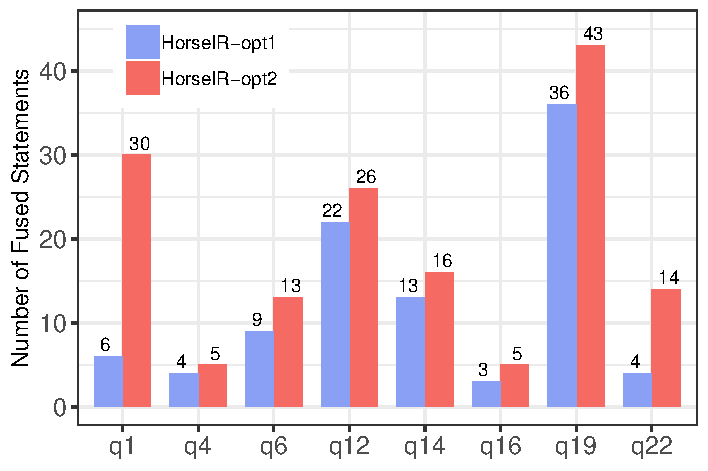
\includegraphics[width=.9\columnwidth]{./src/figure/bar-number.pdf}
\caption{Number of element-wise fused statements in HorseIR-opt1 and our new fusion in HorseIR-opt2.}
\label{fig:opt_number}
\end{figure}

\refFig{fig:opt_number} shows the the number of fused statements using
element-wise fusion in HorseIR-opt1 and the more general function fusion in
HorseIR-opt2.  Note that we do not show pattern-based fusion because both
HorseIR-opt1 and HorseIR-opt2 use the same patterns. 

We can see that our approach always fuses more statements than HorseIR-opt1.
For q1 and q22, there exist a large set of list-related statements that can be
fused together without the need of using patterns.  Furthermore, our optimizer
performs a fair amount of fusions with mixed function types, such as
element-wise and reduction functions. 

However, as we have seen in the previous analysis, fusing is not always
beneficial. For instance, in q22, we perform many more fusions than
HorseIR-opt1, but the loops have now complex expressions which actually results
in worse performance compared to the HorseIR-opt1. 



%%% In the query q1, the number of patterns are significantly reduced because a set
%%% of fusion nodes can be further merged into a single loop due to the same loop
%%% structure.  In q6, the pattern for common masks are removed because the result
%%% of boolean selection will be reduced into a single number so that their the
%%% intermediate results should be discard.


%%% \begin{table}[htbp]
%%% \centering
%%% \caption{Number of statements fused in benchmark queries under two versions of optimizations}
%%% \label{table:opt_number}
%%% \begin{tabular}{|c||c|c|c|c|}
%%% \hline
%%% & \multicolumn{2}{c||}{HorseIR-opt1} & \multicolumn{2}{c|}{HorseIR-opt2} \\ \hline
%%% Query & Patterns & Elementwise & Patterns & Fusion \\ \hline
%%% \hline
%%% q1  & 11 & 2 & 3 & 1 \\ \hline
%%% q4  & 3 & 1 & 2 & 2 \\ \hline
%%% q6  & 1 & 1 & 0 & 1 \\ \hline
%%% q12 & 3 & 5 & 3 & 3 \\ \hline
%%% q14 & 2 & 4 & 2 & 4 \\ \hline
%%% q16 & 5 & 1 & 5 & 2 \\ \hline
%%% q19 & 2 & 6 & 1 & 6 \\ \hline
%%% q22 & 4 & 2 & 2 & 3 \\ \hline
%%% \end{tabular}
%%% \end{table}


\subsection{Discussion}

In summary, we can see that fusion across statements is beneficial in many
cases. However, we can see two situations, where one has to be more careful about
applying fusion. The first is that fusing too many statements might become
sub-optimal. We believe this is due to the increased pressure on register
allocation. Maybe one could create heuristics to determine a maximum number of
statements to be fused. 

The second situation arises when filtering conditions have a high selectivity,
e.g., when only 10 out of a million records qualify. Then the benefit of
avoiding intermediate results is negligible, while the overhead of code fusion
might become a factor. 
If one had enough information about the properties of the actual data, such
unnecessary fusions could be avoided. Therefore, introducing runtime
optimizations in order to decide when to use the optimized code is an
interesting avenue for future research. 




